\documentclass{article}
\usepackage{graphicx}
\usepackage{textcomp}
\usepackage{geometry}
\usepackage{imakeidx}
\usepackage{xcolor}
\usepackage{listings}
\usepackage[utf8]{inputenc}
\usepackage[hidelinks]{hyperref}
\makeindex[columns=3, title=Alphabetical Index, intoc]
\geometry{left=20mm, right=20mm, top=20mm, bottom=20mm}
\colorlet{light-gray}{gray!20}
\hypersetup{
    bookmarks=true,         % show bookmarks bar?
    unicode=false,          % non-Latin characters in Acrobat’s bookmarks
    pdftoolbar=true,        % show Acrobat’s toolbar?
    pdfmenubar=true,        % show Acrobat’s menu?
    pdffitwindow=false,     % window fit to page when opened
    pdfstartview={FitH},    % fits the width of the page to the window
    pdfnewwindow=true,      % links in new PDF window
    colorlinks=false,       % false: boxed links; true: colored links
    linkcolor=red,          % color of internal links (change box color with linkbordercolor)
    citecolor=green,        % color of links to bibliography
    filecolor=magenta,      % color of file links
    urlcolor=cyan           % color of external links
}

\title{Localizzazione con Basestation ITT}
\author{Politecnico di Milano}

\begin{document}

\maketitle

\begin{center}

\includegraphics[scale=0.4]{manual_imgs/Logo_Politecnico_Milano}
\end{center}

\pagebreak

\tableofcontents

\pagebreak


\section{Introduzione}
L'obbiettivo del progetto, qui di seguito illustrato, \'e la \textbf{localizzazione} di un \textbf{target}  in un ambiente noto.
Date le caratteristiche delle apparecchiature utilizzate, l'ambiente in cui viene applicato il progetto \'e di tipo \textbf{indoor}, ovvero al chiuso.

Qui di seguito verranno illustrati tutti gli aspetti rilevanti di questo progetto. Nella Sezione 2 verranno illustrate le apparecchiature utilizzate, le relative propriet\`a e infine il software prodotto per esse.
Nella sezione successiva verr\`a commentato il processo di localizzazione, partendo dal modello teorico sino al prodotto software.

\section{Apparecchiature}
Le apparecchiature utilizzate sono Basestation ITT prodotte da Nuzoo SRL. Esse sono costituite da un'antenna in grado di ricevere e trasmettere a \textit{125Hz} e da un Raspberry Pi, il quale funge da centro di comando.

La frequenza sopracitata permette al segnale di oltrepassare muri ed oggetti con poca attenuazione, per questo \'e stato ritenuto fosse una buona scelta l'applicazione indoor.
Tale segnale per\`o, a causa della frequenza, \'e molto lento; infatti la misurazione attraverso questa frequenza richiede un tempo di circa \textit{400ms}.

Le misurazioni rappresentano la distanza tra la station in questione ed il target; esse avvengono tramite la misurazione della potenza del segnale tra le due apparecchiature citate.
La distanza ottenuta \'e rappresentata da un valore RSSI, ovvero un valore intero tra 31, se molto vicino, e 0 se lontano.
A causa di questa discretizzazione del dominio di valori, si \'e notato che per distanze superiori a 5m le misurazioni tendono ad essere inaffidabili
%Si \'e notato durante esperimenti che il segnale tende ad essere inutilizzabile per distanze superiori ai 5m.

Sperimentalmente \'e stata anche ottenuta una curva che rappresenta la relazione tra la distanza e il valore ottenuto.

%% immagine della curva
\begin{center}
	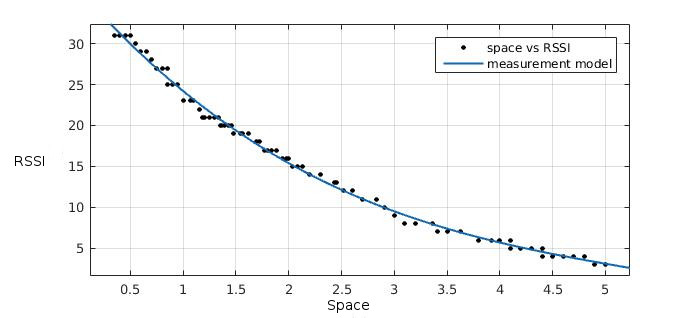
\includegraphics[scale=0.5]{manual_imgs/space_to_rssi}
\end{center}

\subsection{Software}
Come precedentemente detto le station contengono un \textbf{Raspberry Pi}; su tale dispositivo \'e stato installato un sistema Linux, Raspbian. Tale sistema pu\`o essere sostituito con qualsiasi altro, purch\'e sia possibile installare i pacchetti indicati di seguito.

Le station fungono da server per il servizio di localizzazione; esse agiscono come agenti passivi effettuando una misurazione solo se richiesto da un client.
Questa richiesta \'e effettuata mediante il collegamento da parte di un client tramite socket (porta 9111). Non \'e necessario lo scambio di nessuna informazione o chiave; a tal riguardo si sottolinea che non \'e stato considerato nessun aspetto riguardo la sicurezza della comunicazione.

La misurazione richiesta, che come detto richiede \textit{400ms}, viene eseguita inviando tramite seriale il comando \textit{SCANA}.
Questo comando, assieme ad altri, \'e reso disponibile dai produttori al fine di interagire con l'antenna. Esso permette di eseguire una scansione restituendo un valore per tutti i target a portata.

Al fine di utilizzare la seriale si \'e resa necessaria l'installazione della libreria \textbf{wiringPi}; essa viene distribuita gratuitamente ed open-source.

I risultati della misurazione vengono restituiti in formato \textit{json}; \'e stato preferito questo formato rispetto ad xml per una minore verbosit\`a.

\pagebreak

% esempio
\begin{lstlisting}[frame=single, backgroundcolor=\color{light-gray}, basicstyle=\footnotesize\ttfamily, ,caption={An example of message in Json format}]
{
"beacons": 
	[
		{"id_tag":"2022", "rssi":"31"},
		{"id_tag":"2020", "rssi":"15"}
	]
}
\end{lstlisting}


Al fine di poter interagire in maniera efficace e semplice con questo formato, la librearia \textbf{jsoncpp} \'e stata installata.

Una volta trasmessi i dati la connessione viene chiusa dal server, il quale rimane in attesa di un'altra richiesta.


Il software discusso qui sopra \'e stato interamente sviluppato in C++; esso \'e disponibile alla cartella '\textit{code/basestation}'.
Si sottolinea che solo \textit{wiringPi} e \textit{jsoncpp} sono necessarie al corretto funzionamento del server. Gli altri software discussi qui di seguito non sono necessari.

Per semplificare il processo di sviluppo e l'accesso alle station sulle board sono stati anche installati \textit{cmake} e \textit{tightvncserver}.


Le basestation alla loro accensione, automaticamente, lanciano un'istanza del software descritto sopra e danno la possibilit\`a di connessione tramite vnc.
Queste impostazioni permettono il loro utilizzo in stile 'plug-and-play'.


\subsection{Architettura di Localizzazione}

Come detto nella sezione precedente queste apparecchiature richiedono il collegamento ad una rete.\\
Per questo progetto \'e stata impostata la connessione automatica alla rete Wi-Fi, con indirizzo statico.\\
\'e importante sottolineare che \underline{l'indirizzo deve rimanere costante nel tempo}. Di fatto esso rappresenta l'ID della basestation e per tanto \'e associato univocamente alla posizione.


\section{Localizzazione}
La localizzazione del dispositivo, detto target, avviene attraverso un filtro di Kalman esteso (\textbf{EKF}).
Tale procedura \'e stata implementata sotto forma di nodi ROS.
Il software qui descritto \'e possibile trovarlo nella cartella '\textit{code/centralstation}'.

Per poter vedere graficamente la localizzazione viene utilizzato rviz.


\subsection{EKF}
Qui di seguito non verr\`a presentato matematicamente il filtro di Kalman, per dettagli si riferisca a \href{https://en.wikipedia.org/wiki/Extended_Kalman_filter}{ \underline{questa pagina}}.

Come prima implementazione \'e stato creato un modello in Matlab.
Lo stato del EKF rappresenta la posizione stimata del target assieme alla sua velocit\`a, invece come misurazioni vengono utilizzati i valori ricevuti dalle basestation (che ricordiamo varianoo da 31 a 0).\\
Al fine di modellare propriamente il comportamento del filtro in una situazione reale, nel modello Matlab \'e presente un ritarto tra un polling (richiesta di misurazione) e il successivo.


Oltre al ritardo  \'e stata anche introdotta la funzione per la predizione delle misurazioni delle basestation. Tale funzione \'e stata ricavata da misurazione interpolate con un tool Matlab, come descritto precedentemente nella sezione Apparecchiature.

%% immagine inserita sopra


Ovviamente di questa funzione \'e stata anche calcolata la derivata e propriamente utilizzata nel modello.\\
La posizione iniziale del target non \'e nota all'inizio della procedura di tracking, pertanto come punto di partenza viene utilizzata la basestation ritenuta pi\`u vicina.

Il modello citato sopra \'e disponibile nella cartella 'matlab', il file principale \'e 'main.m'. \\


Con tale modello si \'e ottenuto un errore teorico di circa 1-1.5m. Questo risultato ha confermato che, sia il modello che le apparecchiature, possano portare al tracking del target. 


\subsection{Software}
Come anticipato il filtro sopra citato, in seguito, \'e stato implementato sotto forma di nodo, o meglio dire nodi, ROS.

Ogni nodo sviluppato si occupa di gestire un aspetto differente del filtro, qui di seguito si cerca di dare una spiegazione alle scelte implementative effettuate.




\subsubsection{Position Publisher}
Il nodo in questione \'e quello in cui viene effettivamente compiuta la localizzazione del target. Ogni nodo \'e in grado di localizzare un solo target, di cui va specificato il numero identificativo.

Periodicamente il nodo effettua una richiesta, tramite topic, di effettuare delle misurazioni alle '\textit{n}' stazioni pi\`u vicine al target. Si \'e notato che si ottengono buone prestazioni se tale valore non viene limitato, ovvero vengono listate tutte le station.
%Tale valore \'e ovviamente specificabile come parametro '\textit{max\_selection}'. 

Alla ricezione di una misurazione utile, il valore ottenuto viene 'pesato', ovvero ridotto, al fine di non infierire troppo nella stima della posizione. 
Questa modifica avviene sottraendo a valore ricevuto un valore ottenuto in base ad una funziona ricavata sperimentalmente.

%% inserire immagine di tale funzione
\begin{center}
	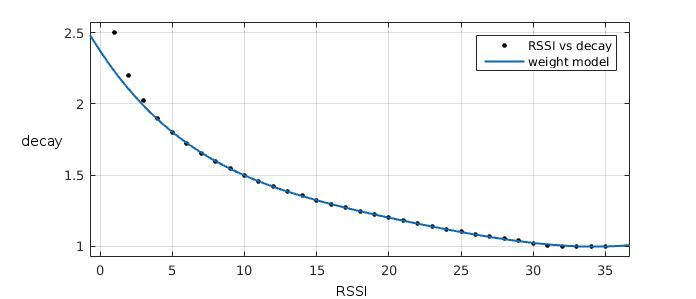
\includegraphics[scale=0.4]{manual_imgs/weight_model}
\end{center}

Non effettuando tale modifica la posizione stimata risulta instabile e pertanto poco utilizzabile.


Una volta pesata la misurazione viene compiuto l'aggiornamento della posizione attraverso il filtro utilizzando le formule classiche.

Si fa notare che \'e possibile definire la varianza delle misurazioni tramite il parametro '\textit{var\_z}'; esso pu\`o anche esser visto come il grado di fiducia delle misurazioni.
Questo parametro \'e stato impostato a 5, per poter contrastare l'attenuazione dovuta ad eventuali muri.


Per semplificare la procedura di lancio del nodo \'e stato creato un launch file.
Nella versione disponibile sono presenti tutti i parametri descritti ed altri necessari con i valori utilizzati durante l'esperimento.\\

Oltre ad i parametri precedentemente indicati, \'e necessario specificarne ulteriori.
\'e richiesta la lista delle Basestation '\textit{basestations}', composta da indirizzo e posizione nello spazio (2D).
Ovviamente l'identificativo del target '\textit{tag}'.
La lista dei coefficienti per il modello di misurazione '\textit{measurement\_model}' e quelli relativi al modello per il peso propriamente la misurazione '\textit{measurement\_weight\_model}'.

Come per altri nodi \'e presente un'opzione di debug, attivabile con il relativo parametro '\textit{debug}'.
Questa funzione mostra graficamente la covarianza della posizione tramite un ellissoide blu, il quale viene trasmesso come Marker tramite il topic '\textit{position\_debug}'.

%% immagine
\begin{center}
	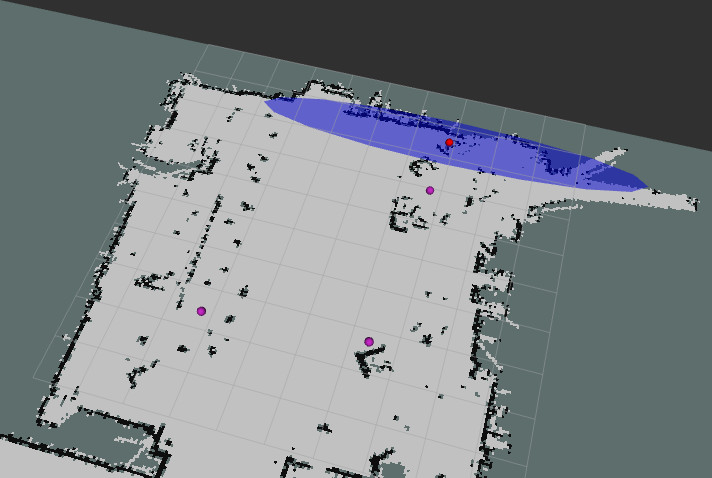
\includegraphics[scale=0.4]{manual_imgs/position_debug}
\end{center}


\subsubsection{Poller}

Al fine di localizzare il target, il nodo deve richiedere alle diverse Basestation di effettuare una misurazione. 
A causa delle limitazioni dei dispositivi non \'e per\`o possibile che pi\`u station effettuino una misurazione contemporaneamente; o quantomeno non \'e espressa questa possibilit\`a nel manuale fornito pertanto \'e stato assunto che ci\`o non sia possibile.

Per evitare di incorrere in problemi di concorrenza e per rendere il sistema di localizzazione scalabile \'e stato definito un nodo ROS, denominato 'poller' il cui compito \'e gestire le richieste di misurazioni.
Per poter rispettare queste premesse il nodo sar\`a l'unico che comunica con le station.

Per evitare di effettuare richieste sempre verso le medesime stazioni, viene utilizzata una lista ordinata od ordered-set.
Tale lista non contiene evidentemente duplicati e memorizza le stazioni in ordine di richiesta secondo la politica FIFO.

\'e possibile comunicare con tale nodo tramite il topic '\textit{measurements\_request}' 
Una volta che la misurazione \'e stata portata a termine la risposta sar\`a disponibile attraverso il topic '\textit{measurements}'.

Nel qual caso una misurazione non vada a buon fine, per esempio la Basestation non risponde, \'e possibile che non venga inviata nessuna risposta.

I messaggi di richiesta sono strutturati come stringa e devono contenere solamente l'indirizzo della station interessata.
Al contrario un messaggio di risposta \'e strutturato in maniera che sia possibile contenere pi\`u misurazioni, o meglio misurazioni per diversi target.
Il messaggio inviato sar\`a del tipo '\textit{MeasurementList}' e conterr\`a i seguenti campi:

\begin{itemize}
	\item Header header $\,\to\,$ contente le informazioni di base;
	\item string basestation $\,\to\,$ contenete l'indirizzo della station da cui arrivano le misurazioni;
	\item Measurement[ ] $\,\to\,$ data contente tutte i dati ottenuti dalla misurazione.
\end{itemize}

Analogamente il sotto-messaggio Measurement \'e composto come segue:
\begin{itemize}
	\item string tag $\,\to\,$ corrispondente al tag del target a cui corrisponde la misura;
	\item uint8 measurement $\,\to\,$ il valore della misurazione ottenuta.
\end{itemize}


Quindi ogni messaggio pu\`o contenere misurazioni relative a diversi target ma provenienti da una sola station.

Analogamente al nodo precedente per facilitarne l'uso, \'e stato creato un launch file.

Questa volta l'unico parametro richiesto sono gli indirizzi delle basestation disponibili nell'ambiente, '\textit{basestations}'.

Opzionalmente \'e possibile impostare un parametro per mostrare messaggi di debug.


\subsubsection{Map Publisher}
Il nodo che si sta per analizzare viene utilizzato solo per mostrare la mappa dell'ambiente.
Infatti non \'e indispensabile che questo nodo sia attivo per il tracking, ne codice \'e stato sviluppato per esso.

Come per i nodi precedenti anche per questo \'e stato preparato un launch file, questa volta i parametri da personalizzare riguardano unicamente la mappa da utilizzare.



\subsubsection{Measurement Debug}
Quest'ultimo nodo \'e utilizzato a scopo di debug.

Esso mostra, graficamente, circonferenze rappresentanti la misurazione effettuata dalla relativa Basestation. Per fare questo viene inviato un messaggio di tipo Marker sul topic '\textit{measurement\_debug}'.
Le misurazioni sono ottenute dal topic '\textit{measurements}'.

Si fa notare che non viene alterato in alcun modo il valore della misurazione, rappresenta quindi il valore utilizzato per la correzione dal filtro prima che venga pesato.

Il colore di queste circonferenze \'e personalizzabile tramite parametro ROS '\textit{colors}', in cui vanno specificato il tag e il rispettivo colore RGB da associare.

Inoltre \'e necessario specificare la lista dei coefficienti del modello da utilizzare per ottenere tali circonferenze '\textit{debug\_model}' e il valore '\textit{alpha}' del colore da mostrare.

Anche in questo nodo \'e \underline{necessario} specificare la posizione delle Basestation nello spazio.

\begin{center}
	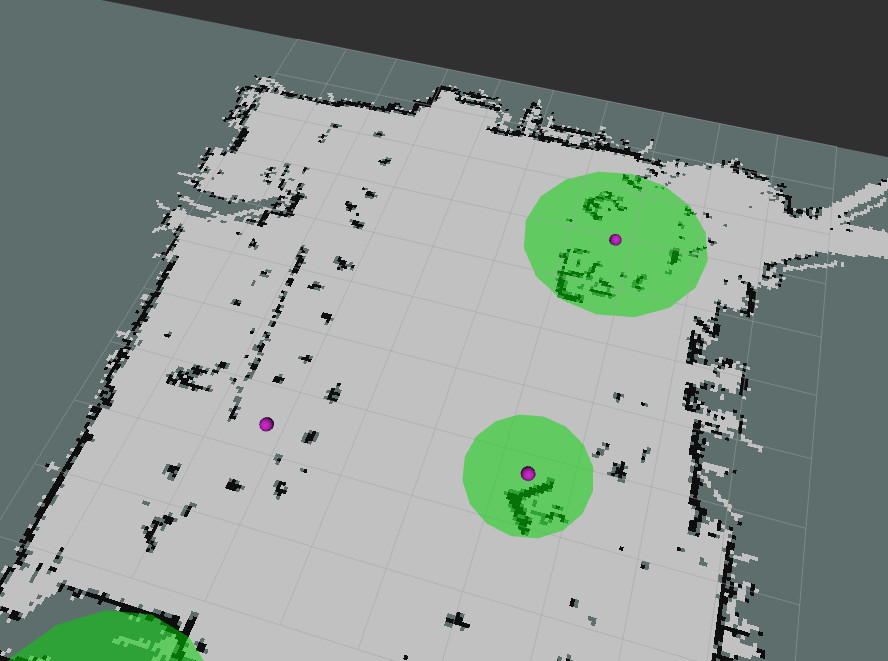
\includegraphics[scale=0.4]{manual_imgs/measurement_debug}
\end{center}


\subsubsection{Configurazione per Rviz}
Qui di seguito verr\`a illustrato brevemente come visualizzare graficamente il risultato della procedura di tracking mediant rviz.

Per prima cosa \'e necessario lanciare tutti i nodi illustrati precedentemente, quindi lanciare rviz.

Al fine di mostrare la mappa dovr\`a essere inserita un apposito elemento \textbf{Map}, il cui topic dovr\`a essere impostato su '\textit{/map}'.

Al fine di mostrare le posizioni delle Basestation e del target nella mappa devono essere inseriti due elementi di tipo \textbf{PointStamped}. \\
Il primo rappresenter\`a le station e andr\`a impostato sul topic '\textit{/basestation}' e aumentato il parametro HistoryLength al numero di station presenti sulla mappa.\\
Il secondo invece rappresenter\`a il target; questa volta il topic da utilizzare sar\`a '\textit{/target\_id}', dove id dovr\`a essere sostituito con il numero relativo al target.
Si consiglia inoltre di cambiare il colore per differenziarlo da quello delle station.

Infine per mostrare i Marker di debug \'e necessario aggiungere due elementi \textbf{Marker}.
Il primo riguarder\`a la posizione e dovr\`a essere impostato sul topic '\textit{/position\_debub}', mentre il secondo su '\textit{/measurement\_debub}'.
Si fa notare che in entrambi i casi i Marker svaniranno dopo 5 secondi; affinch\'e permangano \`e necessario un respawn continuo.



%% aggiungere qualche immagine del 'prodotto finito'



\section{References}
\begin{itemize}
	\item wiringPi http://wiringpi.com/
	\item Extended Kalman Filter https://en.wikipedia.org/wiki/Extended\_Kalman\_filter
\end{itemize}

\printindex

\end{document}
